\chapter{Estado del arte}\label{CAP2}


\section{Introducción a la robótica}
    La robótica es la ciencia y la tecnología que se ocupa del estudio y funcionamiento de los robots a través del diseño, manufactura y aplicación de estos. El objetivo de la robótica es diseñar un robot eficiente. Los robots están siendo cada vez más eficientes a causa de que los creadores e investigadores se enfocan en que estos puedan pensar y aprender por si solos, para ello implementan la tecnología llamada con inteligencia artificial.
    
    \begin{figure}[htb]
        \centering
        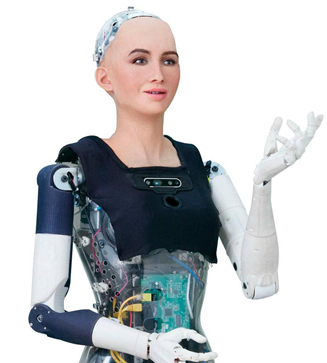
\includegraphics[width=0.4\linewidth]{Main/Chapter2/Images2/Robot-humanoideSophiaIA.png}
        \caption{Robot humanoide Sophia, IA}
        \label{f:Cap2_general_1}
    \end{figure}   
    
    La palabra robot fue usada por primera vez en el año 1921 en la obra de teatro R.U.R (Rossums Universal Robots) creada por el escritor checo Carel Capek (1890 - 1939). El origen etimológico de la palabra es robota, que significa en checo trabajo forzado o esclavo. Posteriormente se emplea la palabra "robótica" en obras de ciencia ficción tales como: Yo Robot (1950) y Robots e imperio (1985) creadas por el escritor y profesor de bioquímica Isaac Asimov (1920-1992).
    
    \newpage
    
    \begin{figure}[htb]
        \centering
        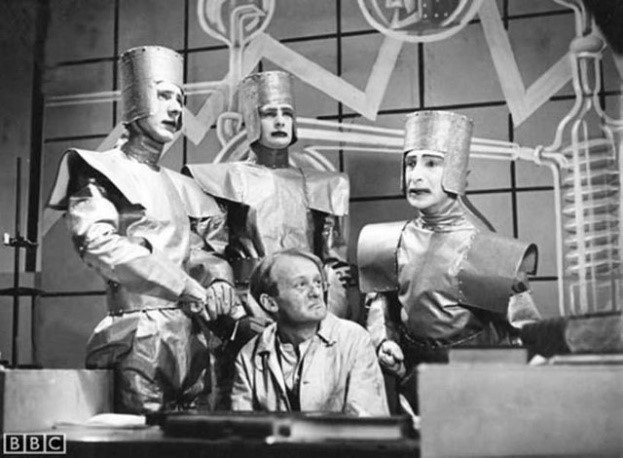
\includegraphics[width=0.6\linewidth]{Main/Chapter2/Images2/Obra-robots.jpg}
        \caption{Obra R.U.R (Robots Universal Rossum) creada por Karel Capek}
        \label{f:Cap2_general_2}
    \end{figure}
    
    Hoy en día los expertos en el área de la robótica y automatización no han llegado a un acuerdo para una definición universal de la palabra robot. Es por esta razón que a continuación se presenta la descripción de un robot respecto al punto de vista de tres instituciones importantes:
    
    \begin{itemize}
    
        \item \textbf{Robot Institute of America (RIA)}: Un robot es un manipulador reprogramable multifuncional diseñado para mover material, partes, herramientas o dispositivos especializados a través de movimientos programados variables para el desarrollo de una variedad de tareas.
        
        \item \textbf{Japanese Industrial Robot Association (JIRA)}: "Un robot de un dispositivo con grados de libertad que puede ser controlado."
        
        \item \textbf{International Federation of Robotics (IFR)}: "Un robot es un mecanismo actuado programable en dos o más ejes con un grado de autonomía, que se mueva en su entorno para realizar tareas previstas.\\
        \textit{Nota 1: Un robot incluye el sistema de control y la interfase con el sistema de control.}\\
        \textit{Nota 2: La clasificación de robot industrial o robot de servicio se hace de acuerdo con la aplicación prevista.}
        
    \end{itemize}
    
    A parir de las tres definiciones anteriores podemos concluir que un robot es un mecanismo programable o re-programable, capaz de interactuar con acciones independientes e inteligentes en un entorno especifico para realizar una variedad de tareas previstas.
    
    En este trabajo de título se estudia un robot de tipo delta. Esta compuesto por tres brazos conectados a una base fija y a otra móvil llamada efector. Al estar los tres brazos conectados a la misma base, la cinemática del robot es cerrada. Los brazos se accionan por medio de actuadores que generalmente son motores. En el efector final se encuentra generalmente herramientas para realizar tareas especificas.
    
    \newpage
\section{Historia de la robótica}
    
    Los robots son una gran noticia hoy en día gracias a las enormes mejoras que han provisto en diversas áreas de la vida de las personas y han abierto un nuevo capítulo en la interacción de humanos y robots para el futuro. Estas enormes mejoras han sido paulatinas, ya que la robótica tiene sus origenes hace miles de años. A continuación, se presentan algunos de los hitos registrados a través de la historia, que han ayudado a la robótica a convertirse en lo que es hoy.
    
 \begin{longtable}[c]{c m{12cm}}
     \label{tab:cap2_efemerides}\\

     \endfirsthead
    
     \hline
     \multicolumn{2}{|c|}{Continuación de la tabla \ref{tab:cap2_efemerides}}\\
     \hline
     \endhead
    
     \hline
     \endfoot
    
     \hline
     \textbf{Simbología}  & \multicolumn{1}{c}{\textbf{Descripción}}  \\\hline\hline
     \textbf{400 A.C} & El matemático y filósofo italiano Arquitas de Tarento hizo una paloma de madera que volaba. \\ \hline
     \textbf{10-70 D.C} & El matemático y científico griego Herón de Alejandría construyó diversos autómatas con forma de ave. Se le atribuye la invención de la primera máquina de vapor, conocida como “aeolipile” y la fuente de Herón. \\ \hline
     \textbf{1452 - 1519} & Leonardo Da Vinci diseño 2 autómatas, el primero consiste en un mecanismo que emulaba el movimiento humano vestido de armadura y el segundo un león mecánico \\ \hline
     \textbf{1947} & Primer manipulador eléctrico servo-controlado, por Goetz. \\ \hline
     \textbf{1952} & Primera máquina de control numérico, que se programa por un lenguaje simbólico Software. \\ \hline
     \textbf{1954} & El primer Robot: manipulador tipo brazo articulado que realizaba una secuencia de movimientos programables, desarrollado por George Devol. \\ \hline
     \textbf{1959} & George Devol conoció a Joseph Engelberger y juntos fundaron en 1960 la empresa Unimation dedicada a la fabricación de robot \\ \hline
     \textbf{1960} & Se produce el primer robot de configuración cilíndrica Versatran, por la compañía American Machine Foundry (AMF) \\ \hline
     \textbf{1961} & Unimation instala el primer Unimate en General Motors en los procesos de fundición; mientras que la Ford Motor Company instala un robot Versatran. \\ \hline
     \textbf{1963} & La compañía Fuji Yusoki Kogyo de Japón desarrolla el primer robot para aplicaciones de palletzing, llamado Palletizer. \\ \hline
     \multirow{2}{*}{\textbf{1968}} & Kawasaki adquiere los derechos de fabricación del Unimate en Japón. Comienza la fabricación e implementación de robots en las industrias de Japón. \\ \cline{2-2}
      & General Motors emplea baterías de robots en el proceso de fabricación de las carrocerías de los coches.\\ \hline
     \textbf{1970} & KUKA, empresa alemana, instala la primera línea de soldadura equipada con robots industriales. \\ \hline
     \textbf{1971} & Se funda la Japanese Industrial Robot Association (JIRA). \\ \hline
     \multirow{2}{*}{\textbf{1973}} & ASEA, empresa sueca, comercializa el primer robot industrial completamente eléctrico, IRB6. \\ \cline{2-2}
      & La empresa KUKA Robotics contruye el primer robot articulado electromecánicamente de 6 ejes nombrado FAMULUS.\\ \hline
     \multirow{2}{*}{\textbf{1974}} & Se funda el Robot Institute of America (RIA), actualmente llamado Robotic Industries Association.  \\ \cline{2-2}
             & Se introduce el primer robot industrial a España. \\ \cline{2-2}
             & Comienza en lenguaje de programación AL del que derivan otros robots posteriormente. \\ \hline
     \textbf{1978} & Unimation, con el desarrollo de Victor Scheinman, introduce el robot PUMA (Programmable Universal Machine for Assembly) con el lenguaje de programacion VAL (Victor’s Assembly Languaje). \\ \hline
     \textbf{1979} & A partir del desarrollo del profesor Hiroshi Makino de la Universidad de Yamanashi de Japón se produce el primer robot SCARA (Selective Compliance Assembly Robot Arm) a manos de Sankyo e IBM. \\ \hline
     \textbf{1980} & Fundación de la Federación Internacional de Robótica (IFR). \\ \hline
     \textbf{1981} & La compañía americana PaR Systems introduce el primer robot Gantry o de plataforma industrial. \\ \hline
     \multirow{2}{*}{\textbf{1984}} & Adept introduce el primer robot SCARA de accionamiento directo llamado AdeptOne. \\ \cline{2-2}
      &  ABB, empresa sueca formada a partir de ASEA, produce el IRB 1000, el robot ensamblador más rápido hasta la fecha. \\ \hline
     \textbf{1987} & Se constituye la Federación Internacional de Robótica con sede en Estocolmo. \\ \hline
     \textbf{1992} & Aparece el robot DELTA, diseñado por el científico suizo Reymond Clavel en su tesis de doctorado. \\ \hline
     \textbf{1994} & Motoman presenta el primer sistema de control de robots (MRC) que proporcionó el control sincronizado de dos robots hasta 21 ejes. \\ \hline
     \textbf{1998} & ABB, basándose en la estructura del robot Delta, desarrolla el Flex-Picker, considerador el robot de selección más rápido del mundo. \\ \hline
     \textbf{1999} & La compañía alemana Reis Robotics, integra una guía de rayo láser integrada dentro de sus brazos robóticos. \\ \hline
     \textbf{2004} & Motoman introduce un sistema de control robótico mejorado (NX100), que provee control sincronizado de cuatro robots hasta 38 ejes. \\ \hline
     \multirow{2}{*}{\textbf{2006}} & La compañía de automatización Comau de Italia presenta el primer Teach Pendant Inalámbrico (WiTP). \\ \cline{2-2}
        & KUKA presenta el primer robot de peso ligero (LWR) conformado por una estructura de aluminio. \\ \hline
     \textbf{2007} & Motoman lanza robots super rápidos de soldadura por arco, que reduce los tiempos de ciclo en un 15\% 
     \\ \hline
     \textbf{2009} &  ABB lanza el robot industrial multipropósito más pequeño, IRB120, que pesa solo 25kg y un alcance de 580mm. \\ \hline
     \textbf{2013} & KUKA presenta un robot diseñado para una colaboración segura humano-robot del área de trabaja llamado LBR iiwa “Leichtbauroboter intelligent industrial work assistant”, que cuenta con 7 ejes. \\ \hline
    \caption{Modificación del trabajo: “Resumen de la evolución de la robótica industrial” por Diego Rendon, Curso de Robótica Industrial, Universidad de ESPE.}
 \end{longtable}
 
    El robot delta fue investigado e inventando en 1985 por el profesor Reymond Clavel y su equipo en el laboratorio de sistemas de robótica de la la École Polytechnique Fédérale de Lausanne (EPFL, Suiza). Ellos comenzaron la investigación del robot delta después de una visita a una fabrica de chocolate. El equipo de Clavel estaba buscando aplicaciones de mano de obra repetitivas para robots, y descubrieron que el empaque de bombones de chocolate era un candidato para este tipo de automatización de alta velocidad y baja carga útil. En ese mismo año se completo el prototipo de robot delta el cual fue patentado. En 1987 la compañía suiza Demareux Robotics and Microtechnology compró una licencia del robot delta y comenzó la producción de robots delta para la industria de empaquetamiento. En 1991 el Dr. Reymond Clavel presentó su tesis doctoral 'Conception d'un robot parallèle rapide à 4 degrés de liberté' y recibió el premio Golden Robot Award, patrocinado por ABB Flexible Automation, por su trabajo innovador y desarrollo del robot delta.


    \begin{figure}[htb]
        \centering
        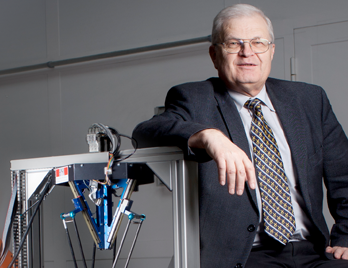
\includegraphics[width=0.36\linewidth]{Main/Chapter2/Images2/Reymond-Clavel-Robot-Delta.png}
        \caption{Reymond Clavel y Robot Delta}
        \label{f:Cap2_general_4}
    \end{figure}
    
    
\newpage    
    
\section{Clasificaciones de robots}
    
    \subsection{Clasificación por generación}

        
        \subsubsection{Primera generación}
            Robots manipuladores. Se caracterizan por programas de control fijos relativamente sencillo de lazo abierto (sin retroalimentación), son capaces de repetir operaciones previamente programadas en ellos, no pueden adaptarse al entorno, por lo que no deben existir perturbaciones externas. Estos robots son los más adecuados en entornos industriales que realizan operaciones repetitivas.
        
        \subsubsection{Segunda generación}
            Robots de aprendizaje. Son adaptativos, pueden operar en entornos variables o parcialmente desconocidos. Estos robots ejecutan una serie de operaciones predefinidas, pero también pueden tener en cuenta los cambios en el entorno y modificar su rutina para realizar sus tareas. Imitan la secuencia de movimientos que ha sido ejecutada previamente por un operador humano. El operador realiza los movimientos requeridos mientras el robot le sigue y los memoriza con ayuda de sensores que recopilan datos.
            
    
            \begin{figure}[htb]
            \centering
            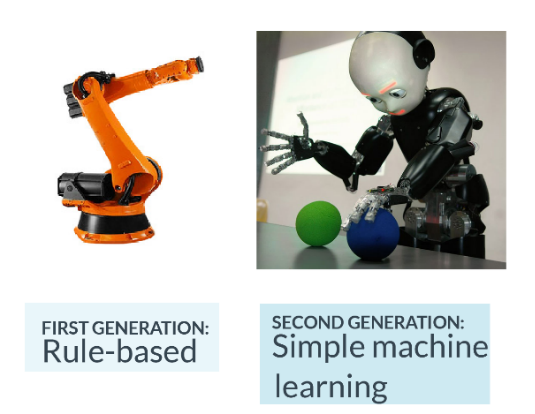
\includegraphics[width=0.9\linewidth]{Main/Chapter2/Images2/Clasificacion-de-los-robots-por-generacion_b.png}
            \caption{Clasificación de los robots por generación}
            \label{f:Cap2_general_5b}
        \end{figure}
        
        \newpage
        
        \subsubsection{Tercera generación}
            Robots con control sensorizado. Los robots cuentan con controladores (computadoras) que, usando los datos o la información recopilada de sus sensores, obtienen la habilidad de ejecutar las ordenes de un programa escrito en alguno de los lenguajes de programación que surgen a raíz de la necesidad de introducir las instrucciones deseadas en dichas máquinas. 
        \subsubsection{Cuarta generación}
            Robots inteligentes. Esta etapa se caracteriza por tener sensores mucho más perfeccionados que mandan información al controlador y la analizan mediante estrategias complejas de control. Incorpora inteligencia artificial totalmente. Esto permite una toma inteligente de decisiones y el control del proceso en tiempo real.
    
    
            \begin{figure}[htb]
            \centering
            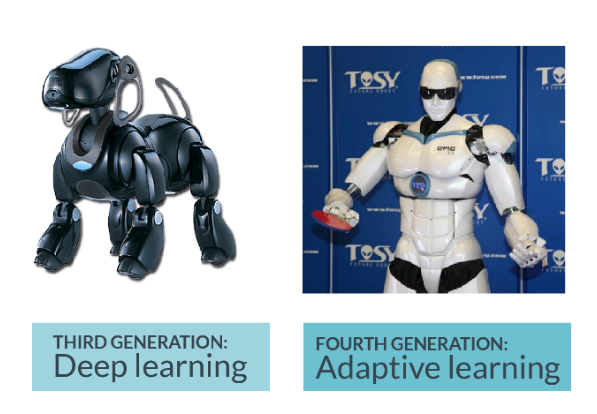
\includegraphics[width=1\linewidth]{Main/Chapter2/Images2/Clasificacion-de-los-robots-por-generacion_a.png}
            \caption{Clasificación de los robots por generación}
            \label{f:Cap2_general_5a}
        \end{figure}
        
        \newpage
        
    \subsection{Clasificación por arquitectura o estructura}
        
        \subsubsection{Poli-articulados}
        La característica principal de este tipo de robots es la de ser sedentarios, aunque algunos tienen desplazamientos limitados. Tienen un espacio de trabajo limitado según uno o más sistemas de coordenadas y tienen un número limitado de grados de libertad
        
        \begin{figure}[htb]
            \centering
            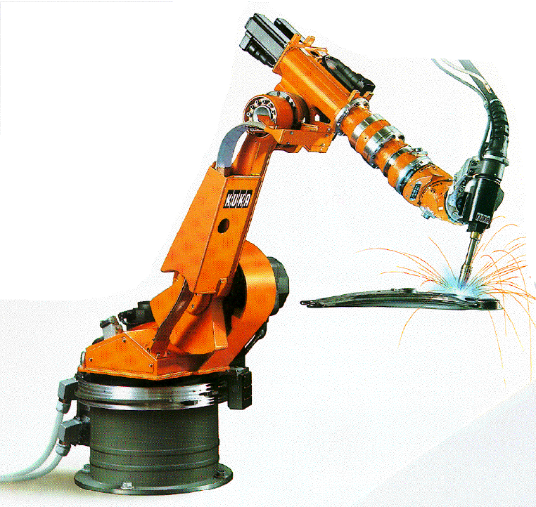
\includegraphics[width=0.4\linewidth]{Main/Chapter2/Images2/Robot-poliarticulado.png}
            \caption{Robot Poli-articulado}
            \label{f:Cap2_general_6}
        \end{figure}
        
        \subsubsection{Zoomórficos}
        La característica principal de este tipo de robot es que imitan los movimientos, desplazamientos y funciones de diversos tipos de seres vivos. Existen dos categorías de robots zoomórficos: no caminadores y caminadores. En la actualidad se encuentran en mayor cantidad los robots caminadores. Estos constantemente están siendo sometidos a experimentos en laboratorios de empresas y universidades para mejorar sus habilidades para realizar de forma más eficiente tareas determinadas. Las aplicaciones de estos robots son esencialmente áreas peligrosas tales como la exploración espacial, estudio de volcanes, fines militares e industrias nucleares. 
        
        \begin{figure}[htb]
            \centering
            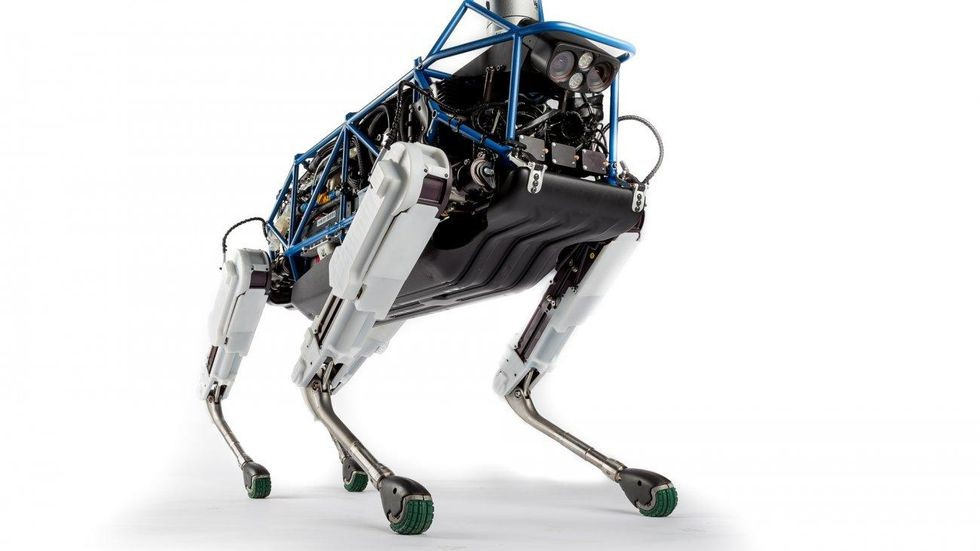
\includegraphics[width=0.5\linewidth]{Main/Chapter2/Images2/Robot-Zoomorico.jpg}
            \caption{Robot zoomórfico}
            \label{f:Cap2_general_7}
        \end{figure}
        
        \newpage
        
        \subsubsection{Móviles}
        Estos robots tienen una capacidad de desplazamiento amplia, basados en carros o plataformas y equipado de un sistema locomotor comúnmente de ruedas. Se desplazan por una trayectoria o camino por medio de un mando a distancia o guiándose a través de la información capturada por los sensores.
        
        \begin{figure}[htb]
            \centering
            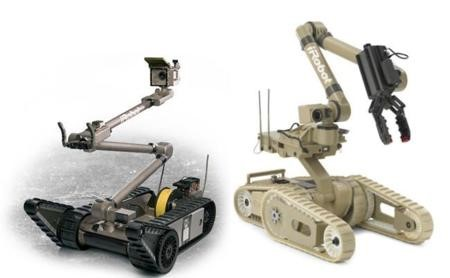
\includegraphics[width=0.4\linewidth]{Main/Chapter2/Images2/Robots-moviles.jpg}
            \caption{Robots móviles}
            \label{f:Cap2_general_8}
        \end{figure}
        
        \subsubsection{Androides}
        La particularidad de este tipo de robots es que son antropomorfos, en otras palabras, que tiene forma o apariencia humana y además imitan algunos aspectos de su conducta de manera autónoma. La mayor dificultad que tienen hoy en día los especialistas de este tipo de robots es simular el comportamiento cinemático del ser humano, llamado locomoción bípeda. La locomoción bípeda es la habilidad de los seres vivos de caminar sobre sus dos extremidades inferiores.
        
        \begin{figure}[htb]
            \centering
            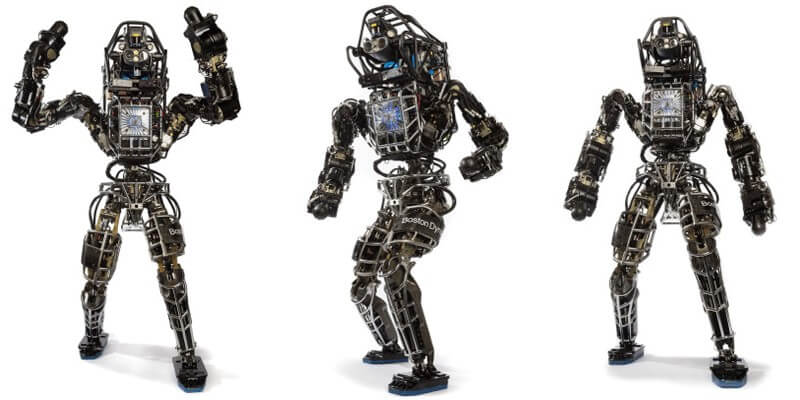
\includegraphics[width=0.6\linewidth]{Main/Chapter2/Images2/Robot-androide.png}
            \caption{Robot androide}
            \label{f:Cap2_general_9}
        \end{figure}
        
        \subsubsection{Híbridos}
        Cuando un robot encaja en 2 o más de las clasificaciones anteriormente dichas se le denomina hibrido. 
        \newpage

    
    \subsection{Clasificación por su movimiento}
    
        \subsubsection{Robots articulados}
        
        El robot articulado es uno de los tipos más comentados de robots industriales. Se asemeja a un brazo humano en su configuración mecánica. El brazo está conectado a la base con una articulación giratoria. Las articulaciones pueden ser paralelas u ortogonales entre sí. Los robots articulados que tienen seis grados de libertad son los robots industriales más utilizados, ya que el diseño ofrece la máxima flexibilidad.
        
        \begin{figure}[htb]
            \centering
            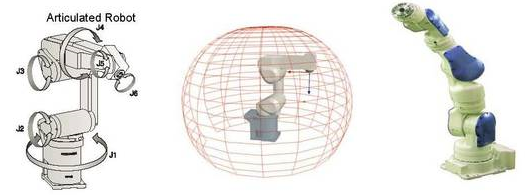
\includegraphics[width=0.9\linewidth]{Main/Chapter2/Images2/Robot-articulado.png}
            \caption{Robot Articulado}
            \label{f:Cap2_segunMovimiento_articulado}
        \end{figure}
        
        \subsubsection{Robots cartesianos}
        
        Los robots cartesianos también se denominan robots rectilíneos y tienen una configuración rectangular. Estos tipos de robots industriales tienen tres articulaciones prismáticas para proporcionar movimiento lineal al deslizarse sobre sus tres ejes perpendiculares (X, Y, Z). 
        
        \begin{figure}[htb]
            \centering
            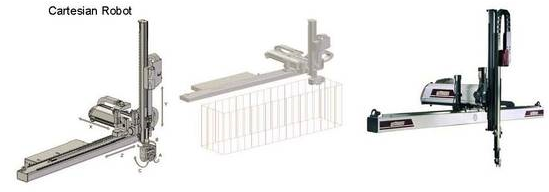
\includegraphics[width=0.9\linewidth]{Main/Chapter2/Images2/Robot-cartesiano.png}
            \caption{Robot Cartesiano}
            \label{f:Cap2_segunMovimiento_cartesiano}
        \end{figure}
        
        \newpage

        
        \subsubsection{Robots SCARA}
        
        Los robots SCARA son robots que pueden hacer 3 traslaciones más una rotación alrededor de un eje vertical. Los ejes rotativos se colocan verticalmente, y el efector final unido al brazo se mueve vertical. Por la configuración de los brazos de SCARA, son flexibles en los ejes XY y rígidos en el eje Z. Los robots SCARA se especializan en movimientos laterales y se utilizan principalmente para aplicaciones de ensamblaje. 
        
        \begin{figure}[htb]
            \centering
            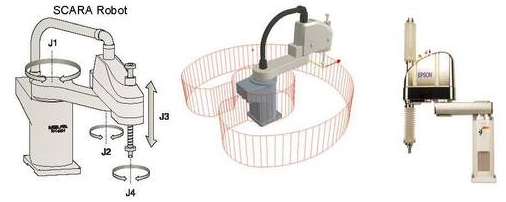
\includegraphics[width=0.9\linewidth]{Main/Chapter2/Images2/Robot-SCARA.png}
            \caption{Robot SCARA}
            \label{f:Cap2_segunMovimiento_scara}
        \end{figure}
        
        \subsubsection{Robots delta}
        
        Los robots delta también se les llama robots paralelos, ya que consiste en enlaces de unión paralelos conectados con una base fija común. Debido al control directo de cada junta sobre el efector final, el posicionamiento de este último se puede controlar fácilmente con sus brazos, lo que resulta un robot de operación de alta velocidad. El espacio de trabajo de los robots delta tienen forma de cúpula. Estos robots se utilizan generalmente para aplicaciones de pick and place.
        
        \begin{figure}[htb]
            \centering
            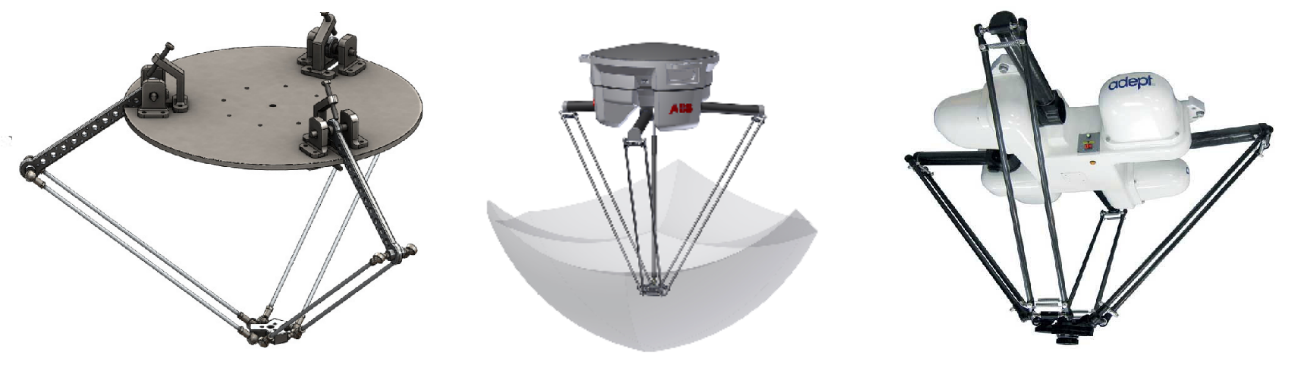
\includegraphics[width=0.9\linewidth]{Main/Chapter2/Images2/Robot-delta.png}
            \caption{Robot delta}
            \label{f:Cap2_segunMovimiento_delta}
        \end{figure}
        
         \newpage

        
        \subsubsection{Robots cilíndricos}
        
        Los robots cilíndricos tienen al menos una junta giratoria en la base y al menos una junta prismática que conecta los enlaces. Estos robots tienen un espacio de trabajo cilíndrico con un eje pivotante y un brazo extensible que se mueve verticalmente y deslizándose. Por lo tanto, los robots con configuración cilíndrica ofrecen un movimiento lineal vertical y horizontal junto con un movimiento giratorio sobre el eje vertical.
        
        \begin{figure}[htb]
            \centering
            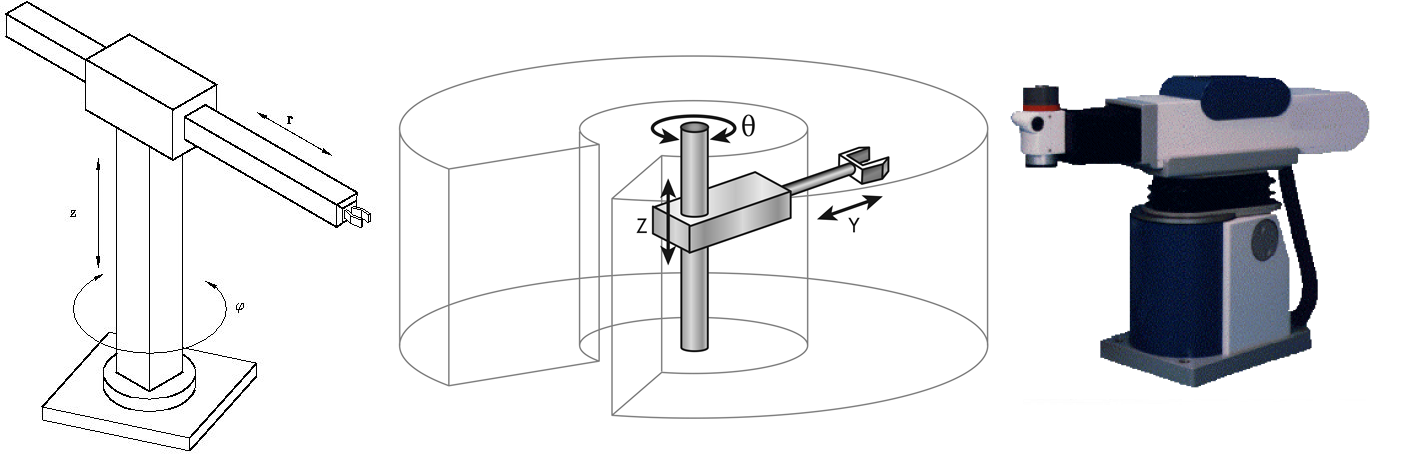
\includegraphics[width=0.9\linewidth]{Main/Chapter2/Images2/Robot-cilindrico.png}
            \caption{Robot cilíndrico}
            \label{f:Cap2_segunMovimiento_cilindrico}
        \end{figure}
        
        \subsubsection{Robots polares}
        
        También llamados robots esféricos, en esta configuración el brazo está conectado a la base con una junta giratoria y una combinación de dos juntas rotativas y una junta lineal. Los ejes forman un sistema de coordenadas polares y crean una envoltura de trabajo de forma esférica.
        
        \begin{figure}[htb]
            \centering
            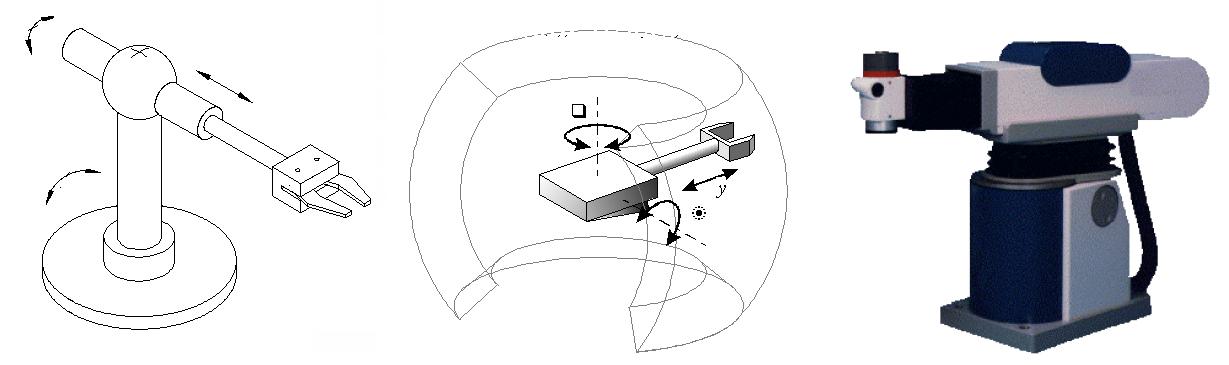
\includegraphics[width=0.9\linewidth]{Main/Chapter2/Images2/robot-polar.png}
            \caption{Robot polar}
            \label{f:Cap2_segunMovimiento_polar}
        \end{figure}
    
                \newpage

    
\section{Estadísticas y aplicaciones}
    Desde
    
